%!TEX root = SysSpec_ClockPendulumAnalyzer.tex
\section{Systemdesign}
    Im Kapitel Systemdesign wird die Umsetzung einzelner Komponenten sowie der gesamte Kontext des \documenttitle\ erklärt.
        \subsection{Kontextdiagramm}
        Der \documenttitle\ Kontext wird mittels untenstehendem Diagramm dargestellt. Das Projekt umfasst ein tinyK20 als Hardware Counter, ein \rpi\ als Recheneinheit und ein Sensor Board auf dem ein Infrarotsensor montiert ist.\\
        Für die Benutzerinteraktion wird ein UserInterface definiert und ein Web Client erstellt. Das UserInterface ermöglicht es weitere Benutzerschnittstellen an den \documenttitle\ zu hängen. Zum Beispiel eine Qt Applikation.
        \begin{figure}[H]
            \centering
            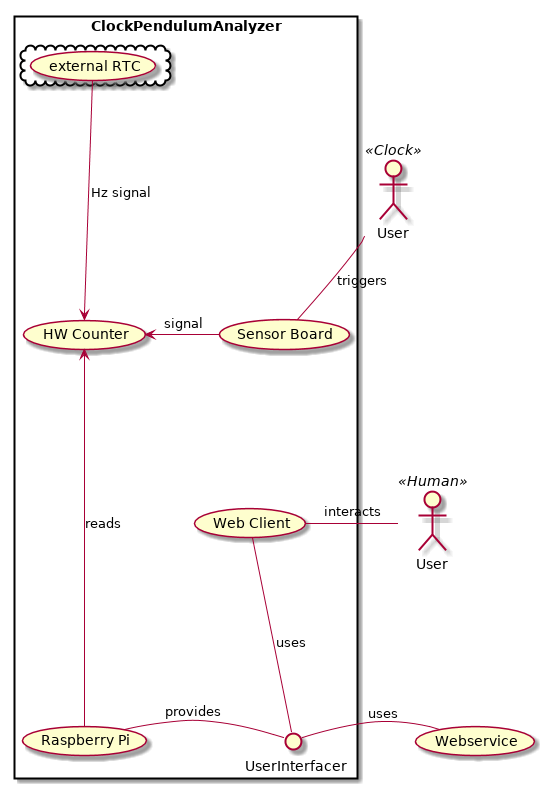
\includegraphics[width=.7\textwidth]{context.png}
            \caption{erweitertes Kontextdiagramm}
            \label{fig:kontext}
        \end{figure}


        \clearpage
        % !TEX root=SysSpec_ClockPendulumAnalyzer
\subsection{Umsetzung des GPIO Zugriff}
Der Zugriff auf die GPIO Pins des \rpi\ wurde mit einer simplen Klasse umgesetzt. Diese Klasse ist verantwortlich für das Exportieren und Unexportieren der Pins.
Dies geschieht bei der Initialisierung der Klasse beziehungsweise beim Dekonstruktor. Dabei wird das Prinzip der ''Resourcenbelegung ist Initialisierung'' (kurz RAII) nicht verletzt.\\
\\
Die Aufgaben des Benutzers sind nur Richtung setzen und dann Lesen bzw. Schreiben der Pins. Die Richtung (Output / Input) kann zur Laufzeit geändert werden.

\subsubsection{Pinbelegung}
Die Pinbelegung auf dem \rpi\ wird in Bild \ref{fig:pi_belegung} gezeigt.
\begin{figure}[H]
    \centering
    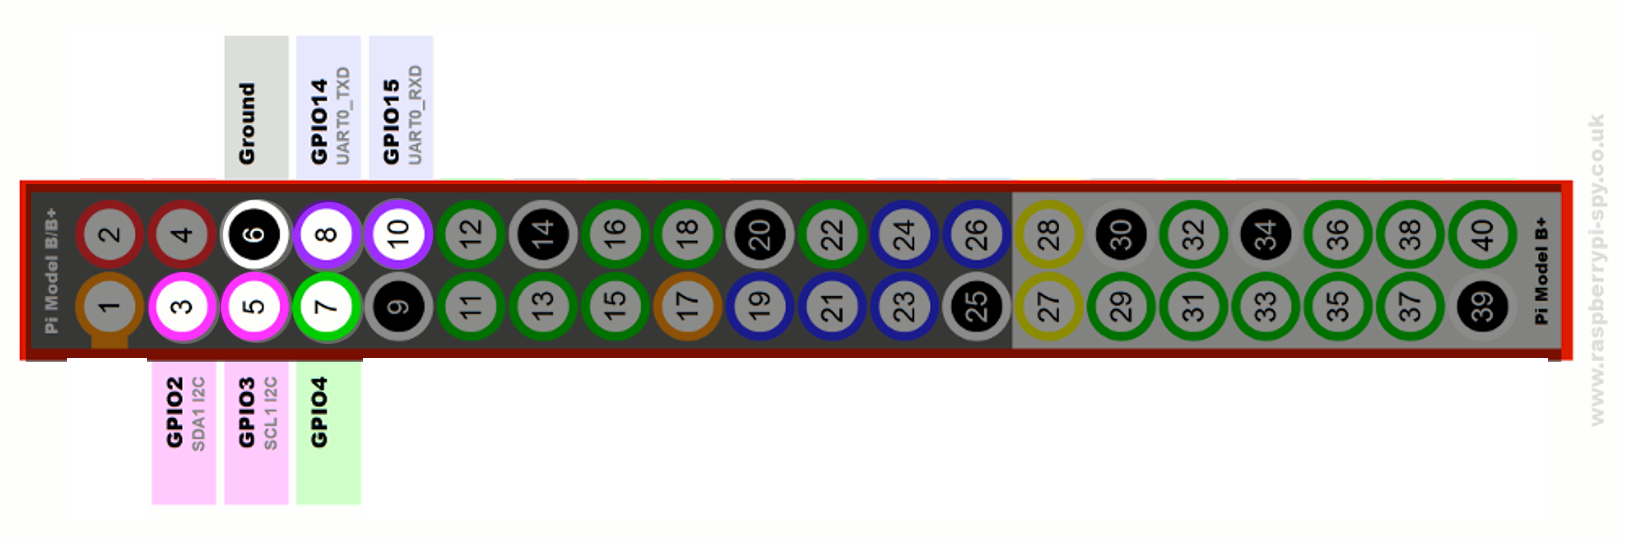
\includegraphics[width=\textwidth]{pinbelegung}
    \caption{Pinbelegung des \rpi\ (Originalbild von www.raspberrypi-spy.co.uk)}
    \label{fig:pi_belegung}
\end{figure}

\noindent Pin 6,8,10,3 und 5 werden nicht durch die GPIO\footnote{General Purpose Input Output} Klasse angesteuert. Diese sind für die UART beziehungsweise \iic\ Kommunikation reserviert, die in den nachfolgenden Kapitel \ref{sec:i2c} und \ref{sec:uart} beschrieben sind.\\\\
Pin 7 dient als Interrupt-Pin für den Zähler. Dieser wird bei Programmstart als High Output Pin gesetzt um damit den Zähler zurückzusetzen. Damit wird erreicht, dass das System auf unterschiedliche Aufstartzeiten reagieren kann und die ganze Messung gleichzeitig starten kann. Der Zähler-Reset wird nur bei Programmstart ausgeführt und danach nicht mehr.

\subsubsection{\iic\ Implementierung}\label{sec:i2c}
Der \iic\ Anschluss läuft über Pin 3 (SDA\footnote{Data Signal}) und 5 (SCL\footnote{Clock Signal}).\\
Für den \iic\ wurde ebenfalls eine abstrahierende Klasse entwickelt. Diese verwendet die bereits vom Linux bereitgestellten Funktionalitäten zum Lesen und Schreiben von \iic-Geräten.\\
\\
Im Kontext des \documenttitle\ ist der \iic\ Bus als Kommunikation zwischen RTC, Zähler und \rpi\ gedacht. 
Dabei wäre das \rpi\ der Master und fordert die anderen zwei Teilnehmer nach ihren Daten.

\paragraph{Aufgetretene Probleme:}
Aufgrund des gewählten Betriebssystem und der dadurch entstandenen Problematik mit der Schnittstelle auf dem \rpi, wird die \iic\ Implementierung nicht beendet.\\
Die Problematik bestand darin, dass die \iic-Geräte auf dem Linux nicht erkannt wurden. Nach mehreren Versuchen die Geräte zu erkennen, wurde entschieden, dass zur Kommunikation eine USB-UART Verbindung aufgebaut wird. Diese Verbindung beinhaltet nur noch die Kommunikation mit dem Zähler des \hwb s. Mehr zum UART ist im folgenden Kapitel \ref{sec:uart} zu lesen.

\clearpage
\subsubsection{UART Implementierung}\label{sec:uart}
Für das Lesen des GPS Signals wird eine UART Kommunikation benötigt.
Aufgrund der \iic\ Problematik wird die GPS UART Verbindung auf den zwei Pins 8 und 10 nicht weiter verfolgt.\\
\\
Dafür wird eine USB-UART Verbindung zum \hwb\ realisiert. Als Übertragungsmedium dient ein micro-USB Kabel und lässt daher nur eine 1-zu-1 Verbindung zu.\\
\\
Der Code basiert auf einer bereits implementierten Lösung aus einem früheren Projekt und wird auf die Bedürfnisses dieser Kommunikation angepasst.\\
Das Lesen des UARTs findet in einem eigenen Thread auf dem \rpi\ statt und empfängt Signale, die vom \hwb\ gesendet werden. Wenn eine Nachricht empfangen wird, wird diese an einer Liste angehängt. Nebenbei läuft der Main-Thread und liest, wenn die Liste einen Eintrag enthält, den Zeitstempel und dessen absolute Zeit aus. Danach wird dieser Eintrag aus der Liste entfernt.
        % !TEX root=SysSpec_ClockPendulumAnalyzer
\subsection{Umsetzung des Clock Update}%TODO rework chapter clock update
Als Clock Update wird der Prozess verstanden, der die Systemzeit des Raspberry aktualisiert.

\subsubsection{Problemstellung}
Das System ist nicht zwingend an einem Internet angeschlossen. Über ein einfaches Lokales Netzwerk kann bereits mit HTTP ein Datenabruf stattfinden. Dies bedeutet, dass sich das Raspberry nicht mittels NTP Protokoll aktuell halten kann.

\subsubsection{Update der Systemzeit}
Als Ablösung für das NTP Protokoll wird das am Hardware Counterboard angehängte GPS Modul verwendet. Über den bereits im Kapitel \ref{sec:uart} beschriebenen UART Anschluss kann die genaue Zeit genommen werden.\\
Dieser Zeitwert vom GPS wird dann für das Setzen der Hardware Clock auf dem Raspberry verwendet.\\
\\
Mit einer genauen Uhrzeit und Datum im System kann ein besser Zeitstempel für den Messwert genommen werden. 

\subsubsection{Systemzeit für Messdaten}
Das System erhält einen kontinuierlichen Zeitstempel bei jedem Messdaten Sampling. Dabei wird während der Zusammensetzung von allen Informationen ein Zeitstempel von der GPS regulierten Systemzeit genommen. Unter Informationen sind Angaben zur absoluten Zeit, Uhrennamen und Datum zu verstehen.\\
\\
Der Zeitstempel ist in einer Form, die für die Datenbank geeignet ist. Näheres zum Format ist dem Kapitel \ref{sec:db_date} zu entnehmen.
        \clearpage
		%!TEX root = Projektdokumentation_ClockPendulumAnalyzer.tex
\subsection{Umsetzung Sensor}
\label{cap:umsetzung_sensor}
	Die Aufbau der Messvorrichtung des Sensors und dessen Anschluss ist nach folgenden Kriterien erfolgt:
	\begin{itemize}
		\item Flexible Positionierung des Sensors in der Höhe.
		\item Kleine Baugrösse um auch in kleineren Uhren messen zu können.
		\item Möglichst einfacher Anschluss mit Sicherung gegen Fehler.
	\end{itemize}
	Für den Betrieb des in Kapitel \ref{cap:sensoren} beschriebenen IR-Sensors sind im Datenblatt die in Abbildung \ref{fig:info_SFH9201} gezeigten Anschlüsse gegeben.
	\begin{figure}[H]
		\centering
		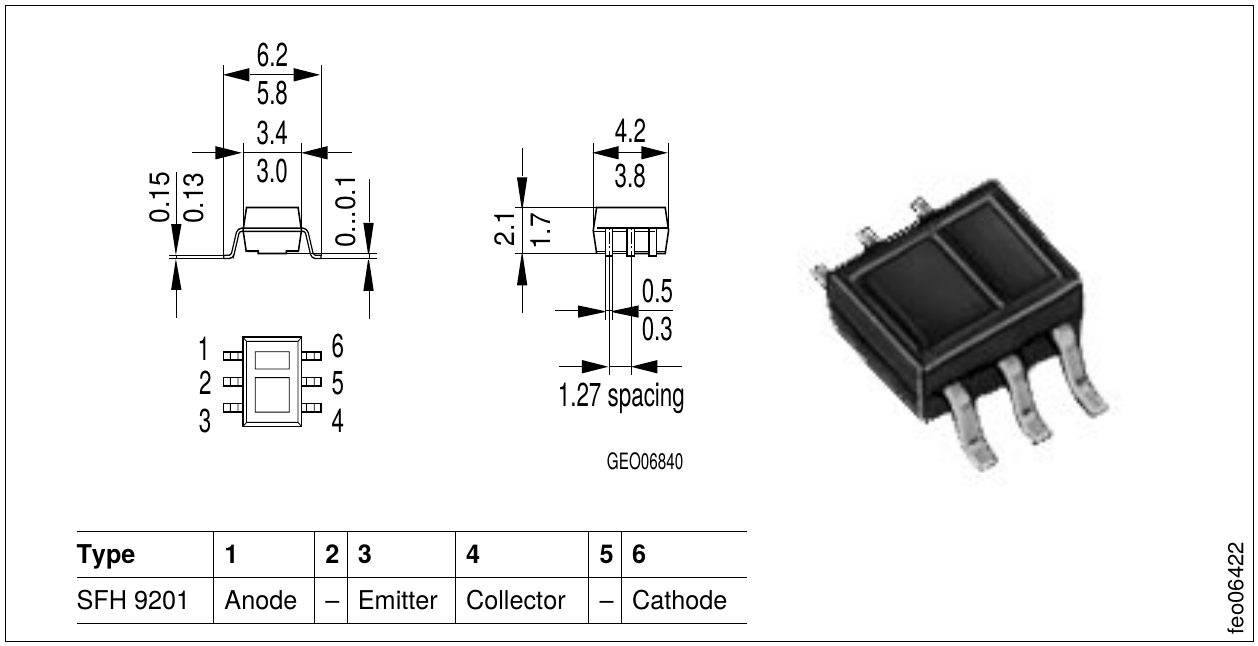
\includegraphics[width=.7\textwidth]{Sensor_layout}
		\caption{Anschlussinformationen SFH9201 (Bildquelle aus Datenblatt)}
		\label{fig:info_SFH9201}
	\end{figure}
	Weiter ist ein Schaltschema gegeben, welches den Grundaufbau der Schaltung vorgibt (Abbildung \ref{fig:schema_SFH9201}).
	\begin{figure}[H]
		\centering
		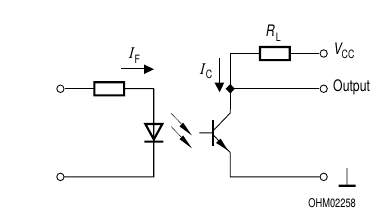
\includegraphics[width=.5\textwidth]{Sensor_Schema}
		\caption{Anschluss-Schema SFH9201 (Bildquelle aus Datenblatt)}
		\label{fig:schema_SFH9201}
	\end{figure}
	\noindent Da die Speisung der Diode und des Collectors in unserem Falle identisch sind, werden drei Anschlüsse benötigt. Eine Speisung mit 3.3V, ein Ausgang, um den Schaltzustand des Sensors zu ermitteln und ein Anschluss für Ground. 
Da es sich um einen analogen Sensor handelt, ist dem Ausgang des Sensors ein Schmitt-Trigger angehängt, welcher die Analoge Spannung in ein digitales Signal umwandelt. 
Das Verhalten des Sensors kann sich, abhängig von der Reflektion des Pendels und des Abstandes zum Pendel, verändern. Deshalb sind sowohl der Vergleichswiderstand des Schmitt-Triggers, sowie der Widerstand der Hysterese des Schmitt-Triggers mittels Potentiometer einstellbar gestaltet. 
Um die Schaltung für jedes Pendel einfach einstellen zu können, is eine grüne LED (D1) angebracht. Diese als visuelle Hilfe. Der Schaltwert ist dabei auf 3.3V, wenn kein Objekt erkannt wird und 0V, wenn ein Objekt erkannt wird. Dementsprechend verhält sich auch die LED. Gemeinsam ist das in Abbildung \ref{fig:schema_sensor} dargestellte Schema entstanden.
	\begin{figure}[H]
		\centering
		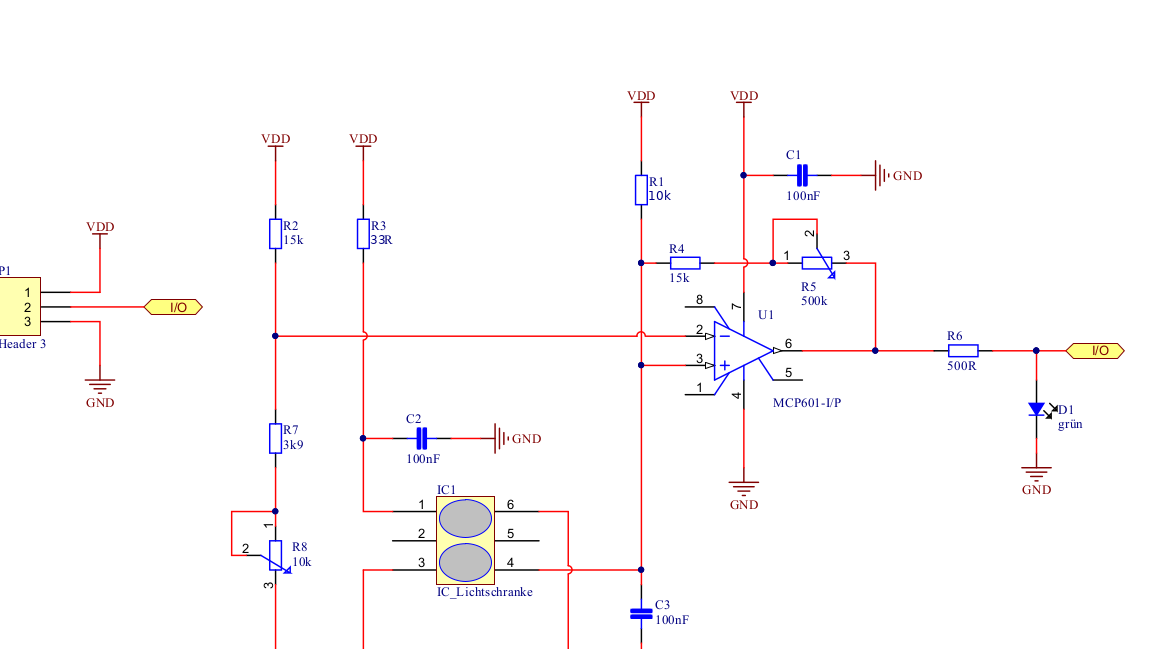
\includegraphics[width=.9\textwidth]{Circuit_Sensor}
		\caption{Ermitteltes Elektroschema für das Sensor-PCB SFH9201}
		\label{fig:schema_sensor}
	\end{figure}
	\noindent Ein falsches Anschliessen des Sensors wird durch das gewählte Steckersystem verhindert. Der Widerstand R1 mit 33$\Omega$ ist der Vorgabe gemäss Datenblatt berechnet. Diese sind:
	\begin{itemize}
		\item 1.65V als maximale und gemessene Spannung $U_{IRD}$ über der IR-Diode
		\item 50mA Betriebsstrom $I_F$
	\end{itemize}
	Ausgehend von einer Speisung $U_S$ von 3.3V ergibt dies folgende Formel:
	\[
		R = \frac{U_S - U_{IRD}}{I_R} = \frac{3.3 - 1.65}{0.05} = 33\Omega
	\]
	Die Werte für die Potentiometer wurden in Zusammenarbeit mit der Elektrotechnik ermittelt. Der 3.9$k\Omega$ Widerstand R7 dient als Minimalwiderstand für die Schwellspannung, welche mit dem Potentiometer R8 justiert werden kann. Diese Einstellung entscheidet, bei wie viel Reflektion ein Pendel registriert wird.
Das Potentiometer R5 dient zum Einstellen, bei welcher Spannung zurückgeschaltet wird um ein Flattern zu vermeiden.
Ein entsprechendes PCB\footnote{Printed Circuit Board} ist an der Hochschule Luzern, Technik \& Archtektur erstellt worden (Abbildung \ref{fig:Sensor_overview}).\\
	\begin{figure}[H]
		\centering
		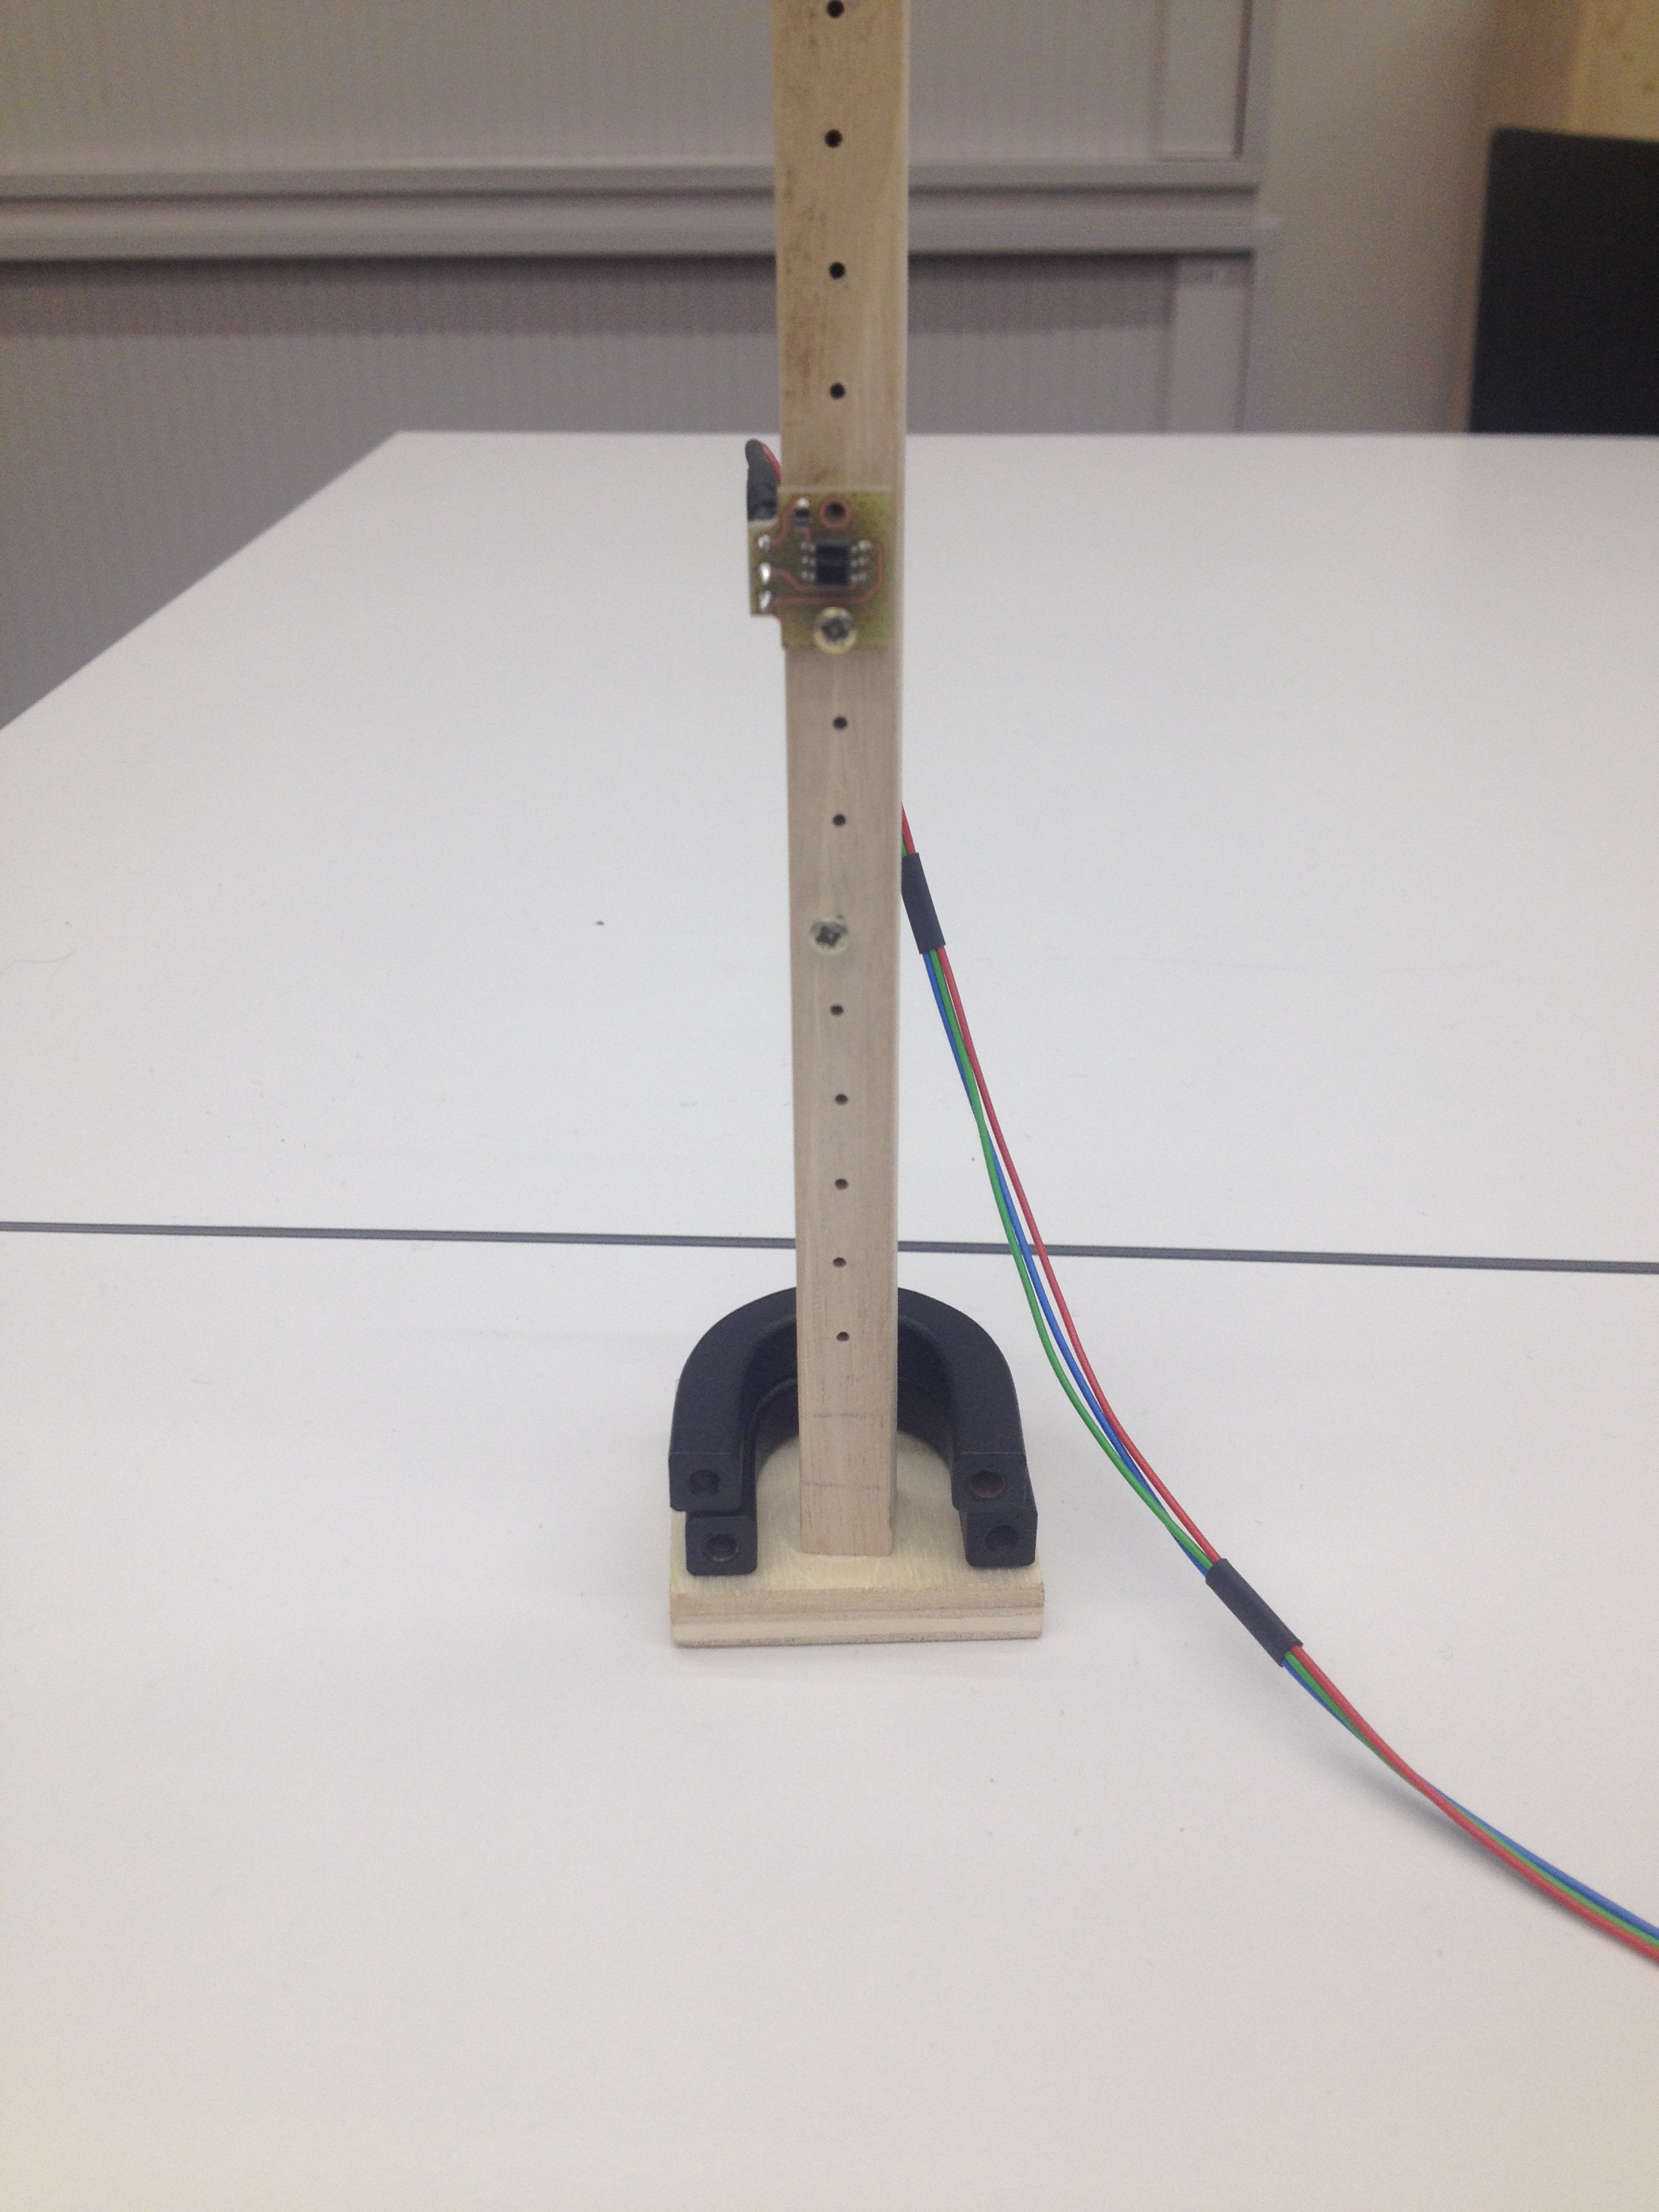
\includegraphics[width=.4\textwidth]{Sensor_overview}
		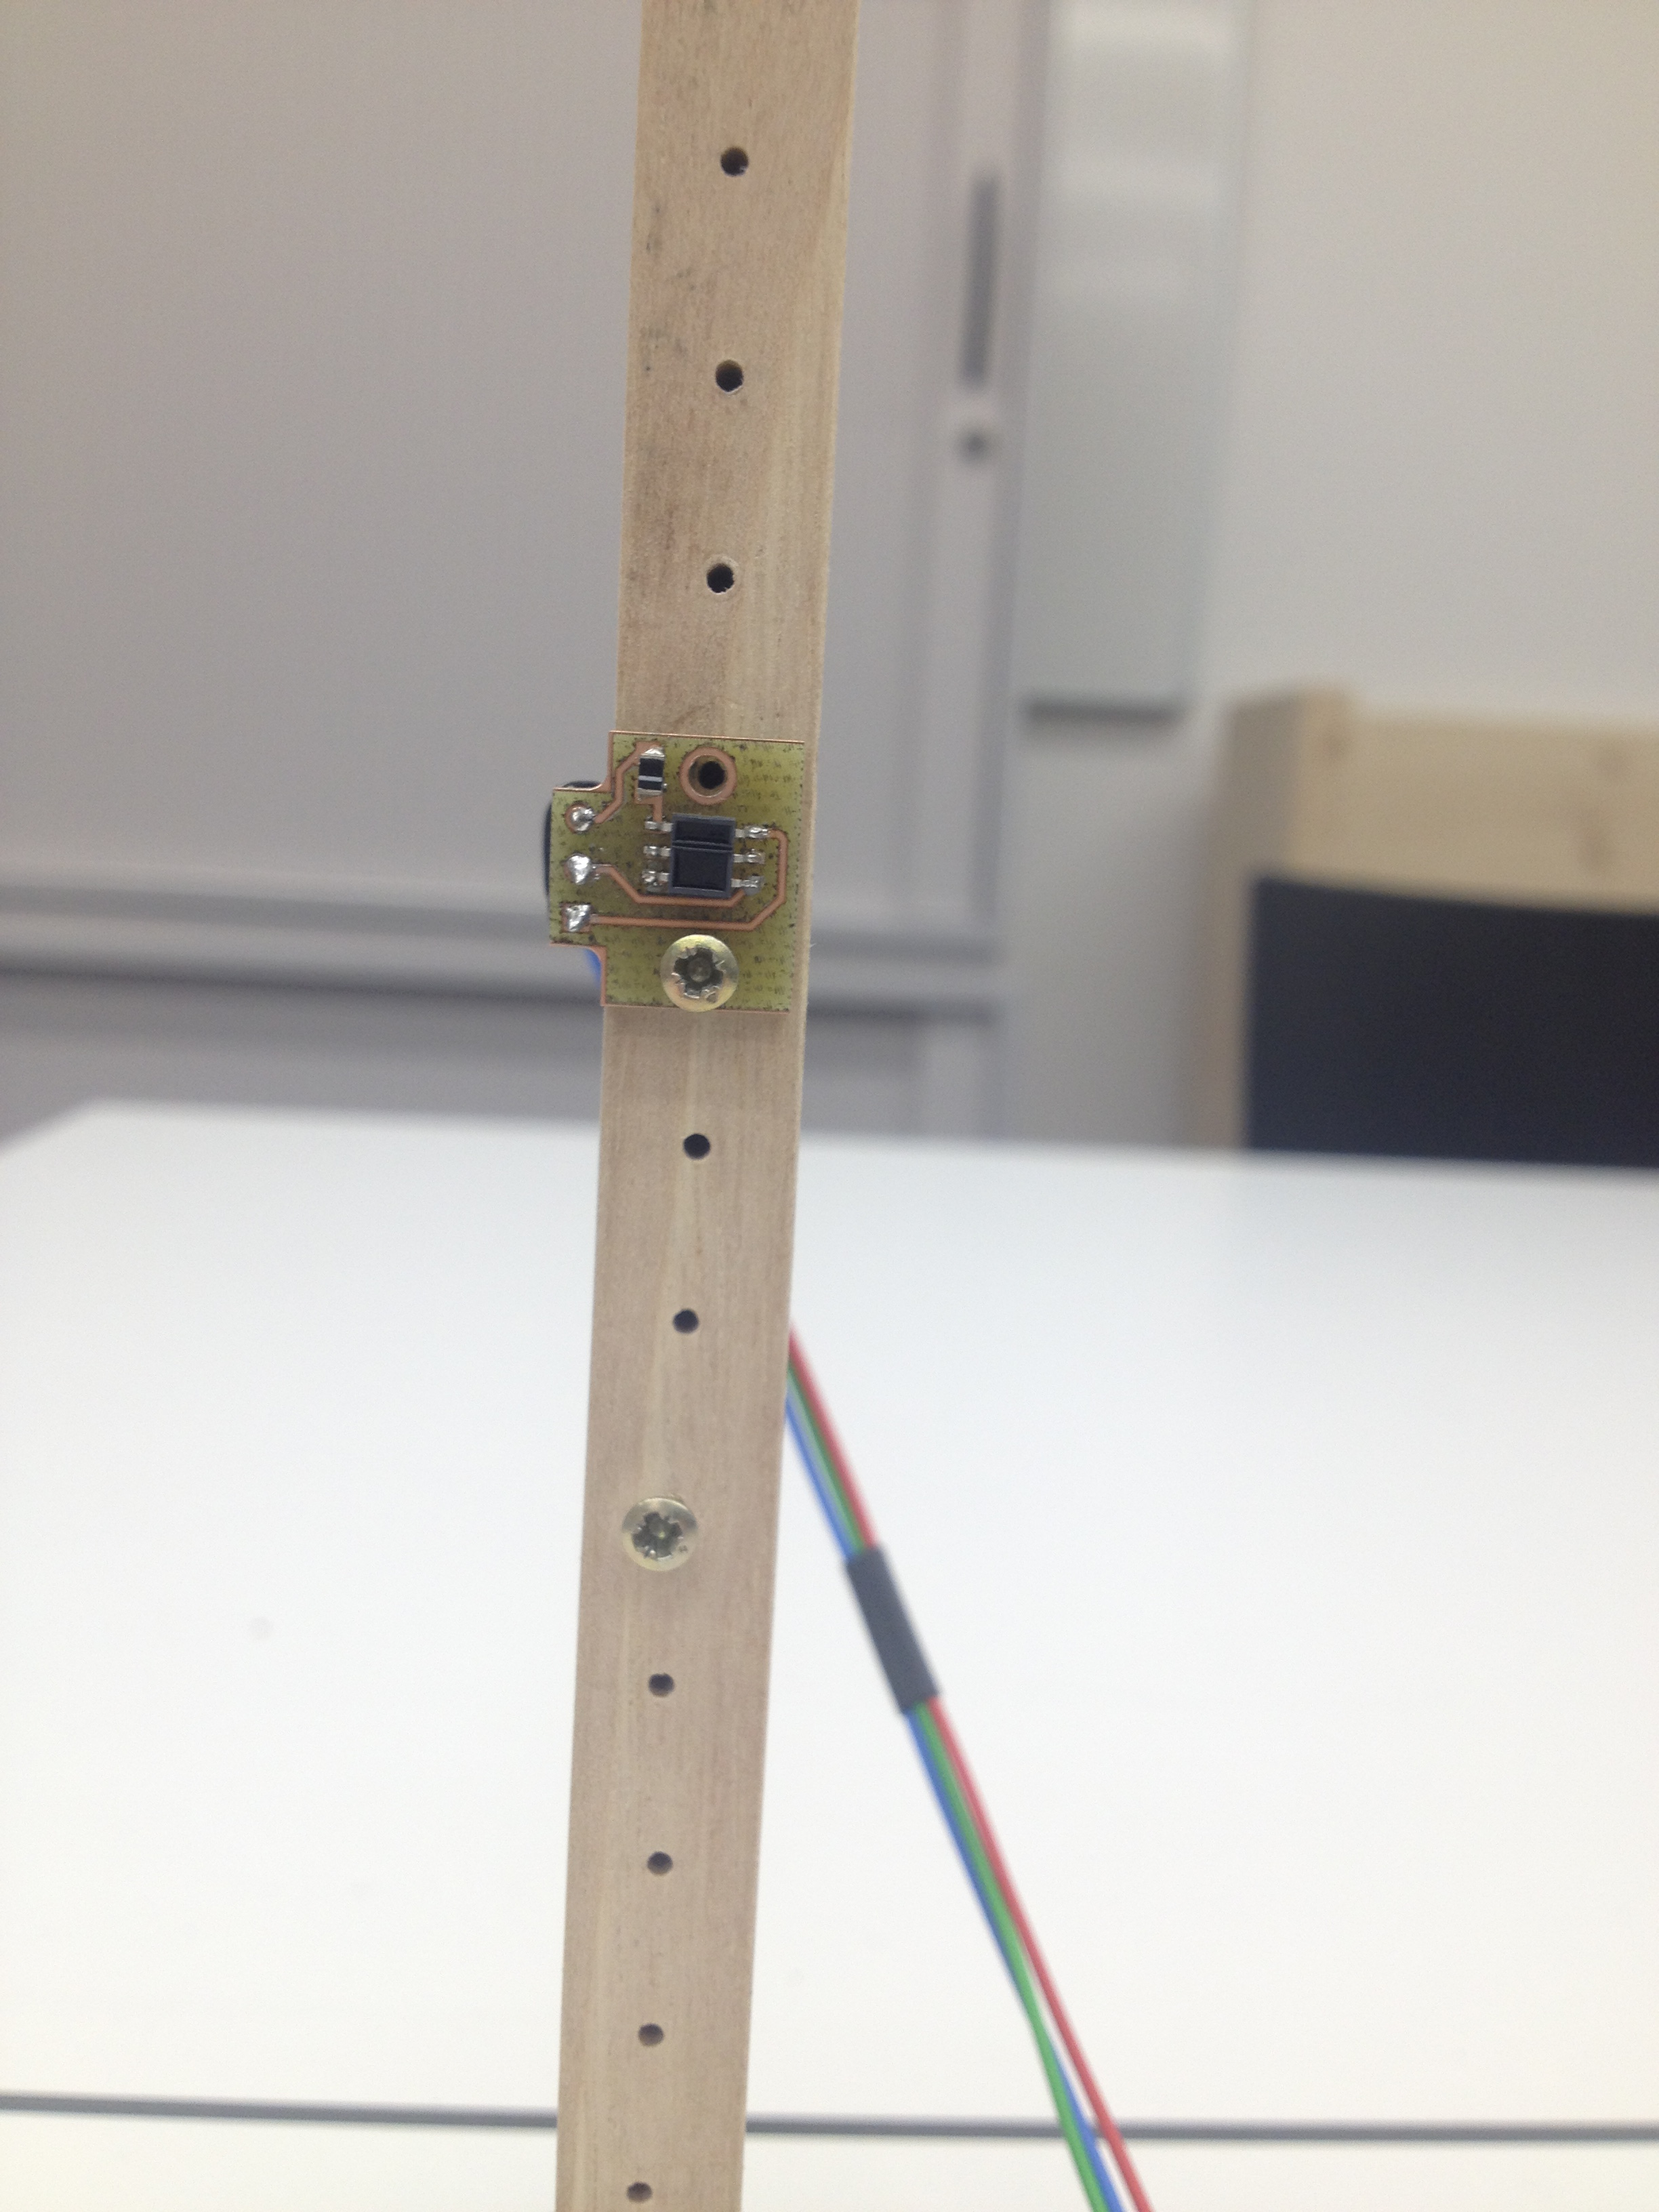
\includegraphics[width=.4\textwidth]{Sensor_Detail}
		\caption{Aufbau des Sensors für die Pendelmessung}
		\label{fig:Sensor_overview}
	\end{figure}
	\noindent Als Stütze für den Sensor dient eine Holzkonstruktion, welche über ein Lochraster von 10mm verfügt, an welchen sich der Sensor befestigen lässt. So können verschiedene Pendellängen und Anordungen abgedeckt werden (Abbildung \ref{fig:Sensor_FullView}). Zwei Gewichte am Fuss verhindern ein Kippen der Konstruktion.
	\begin{figure}[H]
		\centering
		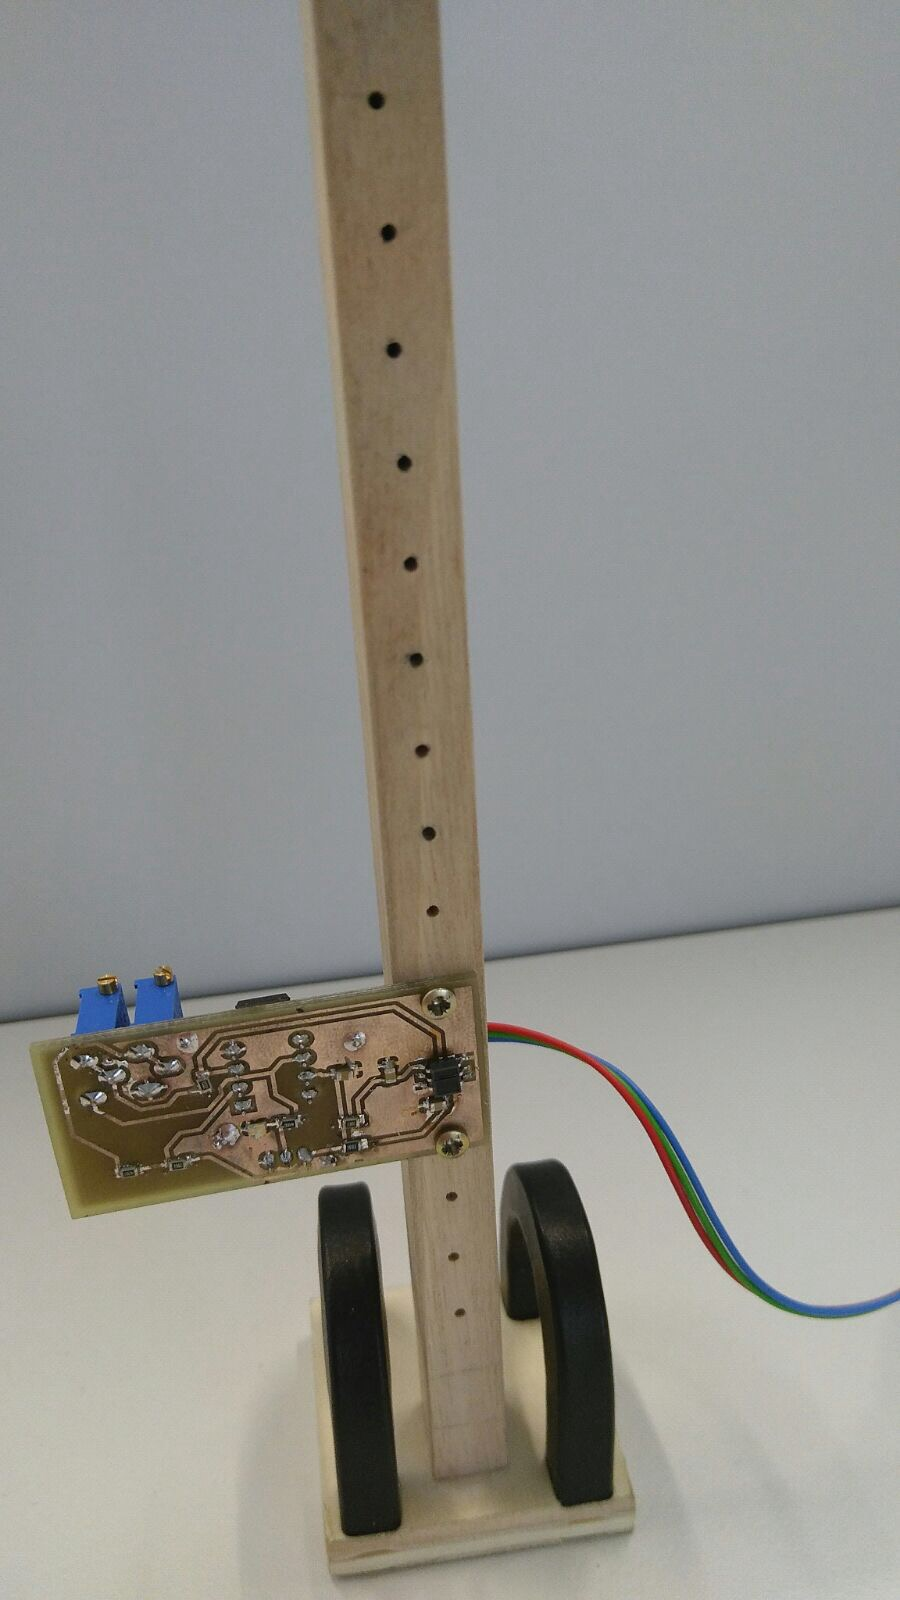
\includegraphics[width=.25\textwidth]{Sensor_FullView}
		\caption{Aufbau des Sensors für die Pendelmessung}
		\label{fig:Sensor_FullView}
	\end{figure}
	\noindent Der Sensor sollte für ein optimales Ergebnis maximal 5mm vom nächsten Punkt am Pendel entfernt angebracht werden. Weiter sollte das Pendel möglichst mittig erfasst werden, um Streuungen zu vermeiden. Die zuvor beschriebene LED (D1 in Abbildung \ref{fig:Sensor_overview} muss konstant aus sein, wenn sich das Pendel vor dem Sensor befindet. 
Der Sensor lässt sich entweder am Rand der Bahn anbringen, dann wird jede Messung erfasst und das Pendel passiert den Sensor nicht vollständig oder mittig, wenn das Pendel den Sensor vollständig passieren soll. Im zweiten Fall muss dann jede zweite Messung verworfen werden, damit das Pendel immer von der selben Seite erfasst wird. Abbildung \ref{fig:sensor_position} zeigt einen optimalen Positionierbereich für den Sensor, innerhalb des roten Rahmens.
	\begin{figure}[H]
		\centering
		\includegraphics[width=.25\textwidth]{sensor_position}
		\caption{Optimale Position des Sensors für die Pendelmessung}
		\label{fig:sensor_position}
	\end{figure}
	\noindent Schwarze, matte Oberflächen werden erst ab einem Abstand von ca. 2mm erkannt. Somit lassen sich Kreispendel messen, wenn mit einem entsprechenden Filzschreiber ein Bereich bestrichen wird, welcher zwischen 6mm und 10mm breit sein sollte.
		%!TEX root = SysSpec_ClockPendulumAnalyzer.tex
\subsection{Umsetzung des Zählers} %TODO Counter Realisierung beschreiben
Der Tick-Conter zwischen den Pendeldurchgängen basiert auf einem Freilaufendem Hardware-Zähler, welcher auf dem Tiny K20 Mikrocontrollerboard läuft, getrieben von dem vorhandenen, termperaturkorrigieren 8MHz Quarz, mittels Hardware-Einstellung des CPU-Blocks auf 12MHz erhöht. Diese Erhöhung beruht rein auf Hardware-Einstellungen, die Genauigkeit wird entsprechend nicht beeinflusst.
Um die Schwankungen des Zählers auszugleichen wird der Sekundenpuls des GPS-Moduls über zwei unabhängige IO-Pins genutzt. Eine Leitung am FIX-Pin des GPS-Moduls angeschlossen, für den Fall, dass keine GPS-Verbindung besteht und eine Zweite am PPS-Pin des GPS-Moduls, falls GPS-Verbindung besteht.
Beide Leitungen funktionieren über einen Interrupt der höchsten Priorität. Falls am PPS-Pin Interrupts eingehen, wird der FIX-Pin ignoriert. Beim Umschalten zwischen GPS-Empfang und keinem GPS-Empfang kann daher ein Fehler entstehen. Im Normalbetrieb werden die Interrupts an den IO-Pins, eingehend vom GPS-Modul, dazu genutzt die Differenz zwischen dem vorigen Zählerwert und dem aktuellen Zählerwert zu bilden und so die effektive Frequenz zu ermitteln. Bei Störungen wird die Referenzfrequenz nicht korrigiert und mit dem letzten Wert weitergearbeitet. Um eine Störung festzustwellen wird geprüft, ob die ermittelte Referenz-Frequenz im erlaubten Bereich von +/-100ppm zum erwartenten Wert abweicht.\\ 
Die Pendeldurchgänge werden über einen weiteren IO-Pin über einen Interrupt der höchsten Priorität ermittelt. Dabei wird jede zweite Messung verworfen, um das Pendel immer von der gleichen Seite zu messen. Der ermittelte Zählerwert wird mit der ermittelten Frequenz verrechnet und über die UART-RS232 Schnittstelle gesendet.\\
Die Verrechnungskorrektur erfolgt über folgende Formel:
\[
	T_{abs} = \frac{T_{measured} \cdot f_{ref}}{f_{real}}
\]
\subsubsection{Genauigkeit Referenzfrequenz TinyK20}
Die Genauigkeit der Referenzfrequenz ist mittels statistischer Methoden ermittelt worden. Dazu sind zwei Versuchstreihen durchgeführt worden. Jeweils zwanzig Vergleiche mit dem FIX-Pin als Sekundenpuls, somit ohne GPS-Verbiundung und 20 Messungen mit dem PPS-Pin als Sekundenpuls. Temperatur und Luftfeuchtigkeit sind mit einem Sensirion SHTC1- Sensor ermittelt worden.
Die Frequenzwerte sind dem Debug-Systems aus dem Kinetis Design Studio entnommen, jeweils mit ca zehn Sekunden Pause zwischen zwei Werten. Die ermittelten Daten sind in Tabelle \ref{tab:testvalues} aufgelistet.
\begin{table}[H]
	\centering
	\begin{tabular}{|l|l|} \hline
		\textbf{Werte ohne GPS-Empfang}	& \textbf{Werte mit GPS-Empfang} \\ \hline
		11980515						& 11980579 \\ \hline
		11980483						& 11980569 \\ \hline
		11980481						& 11980569 \\ \hline
		11980487						& 11980577 \\ \hline
		11980527						& 11980577 \\ \hline
		11980493						& 11980575 \\ \hline
		11980532						& 11980578 \\ \hline
		11980539						& 11980581 \\ \hline
		11980500						& 11980582 \\ \hline
		11980546						& 11980577 \\ \hline
		11980505						& 11980578 \\ \hline
		11980511						& 11980570 \\ \hline
		11980518						& 11980585 \\ \hline
		11980520						& 11980585 \\ \hline
		11980517						& 11980582 \\ \hline
		11980521						& 11980581 \\ \hline
		11980559						& 11980584 \\ \hline
		11980555						& 11980589 \\ \hline
		11980529						& 11980590 \\ \hline 
		11980521						& 11980589 \\ \hline
	\end{tabular}
	\caption{Testwerte jeweils ohne- und mit GPS-Empfang}
	\label{tab:testvalues}
\end{table}
Es sind im Anschluss folgende Untersuchungen erfolgt:
\begin{itemize}
	\item Streuung der Daten mit Hilfe eines Histogramms und Box-Plots
	\item sowie eine Prüfung auf die Verteilung mittels QQ-Plot.
	\item Umgebungstemperatur: 23.74°.
	\item Luftfeuchtigkeit: 27.16%
\end{itemize}
Der Boxplot in Abbildung \ref{fig:freq_boxplot} zeigt auf, dass die Genauigkeit des Sekundenpulses des GPS-Modules deutlich von der Genauigkeit des PPS-Signals abweicht. Im vorhandenen Versuch liegt die Streuung ohne GPS-Empfang bei 78ppm während die Streuung mit GPS noch 21ppm beträgt. Die Zahlen entsprechen der Summe de folgender Fehler:
\begin{itemize}
	\item Signals des GPS-Modules.
	\item Registrierung des Interrupts.
	\item Ungenauigkeit des Hardware-Zählers.
	\item Auswerten des Zählerstandes und Differenzbildung. 
\end{itemize}
	\begin{figure}[H]
		\centering
		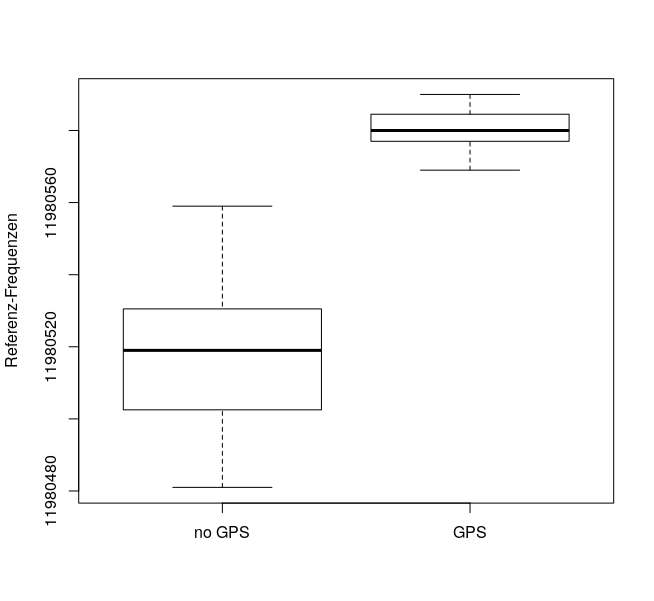
\includegraphics[width=.6\textwidth]{frequencies_boxplot}
		\caption{Boxplot der Versuchsreihen}
		\label{fig:freq_boxplot}
	\end{figure}
%
Weiter kann dem Boxplot entnommen werden, dass die Streuung der Werte gleichmässig um den Median erfolgen und keine Ausreisser vorhanden sind. Dies legt die Vermutung nahe, dass sich die Streuung Normalverteilt verhält, was bedeuten würde, dass sich der Fehler über lange Sicht aufhebt, bis auf eine Konstante Abweichung, welche sich mit der Differenz zwichen Erwartungswert und dem definierten Wert ermitteln lässt. Diese Vermutung ist mit einem Historgramm (Abbildung \ref{fig:freq_histograms}) und einem QQ-Plot (Abbildung \ref{fig:freq_qq_plot}) überprüft worden.
	\begin{figure}[H]
		\centering
		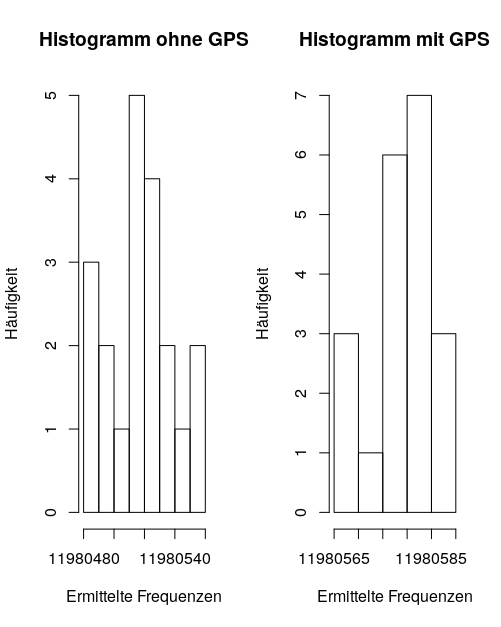
\includegraphics[width=.6\textwidth]{histograms_frequencies}
		\caption{Histogramme der ermittelten Zählerdaten}
		\label{fig:freq_histograms}
	\end{figure}
	Das Histogramm alleine ist bezüglich der Verteilung noch nicht aussagekräftig, dem QQ-Plot kann man anschliessend entnehmen, dass sich die Werte einer Normalverteilung nähern.
	\begin{figure}[H]
		\centering
		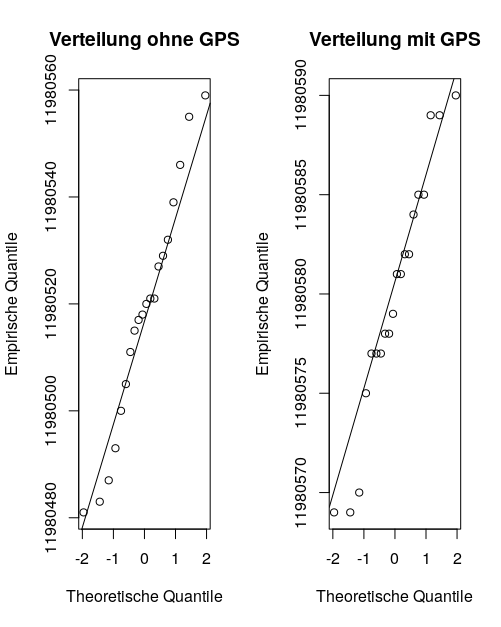
\includegraphics[width=.6\textwidth]{frequencies_qq_plots}
		\caption{QQ-Plots der ermittelten Zählerdaten}
		\label{fig:freq_qq_plot}
	\end{figure}
GPS-Modul und Tiny K20 sind auf einem Board gemeinsam angebracht, ebenfalls auf diesem Board befindet sich die RTC und er Anschluss für den Sensor für die Pendel-Registrierung (Abbildung \ref{fig:hardware_board}).
	\begin{figure}[H]
		\centering
		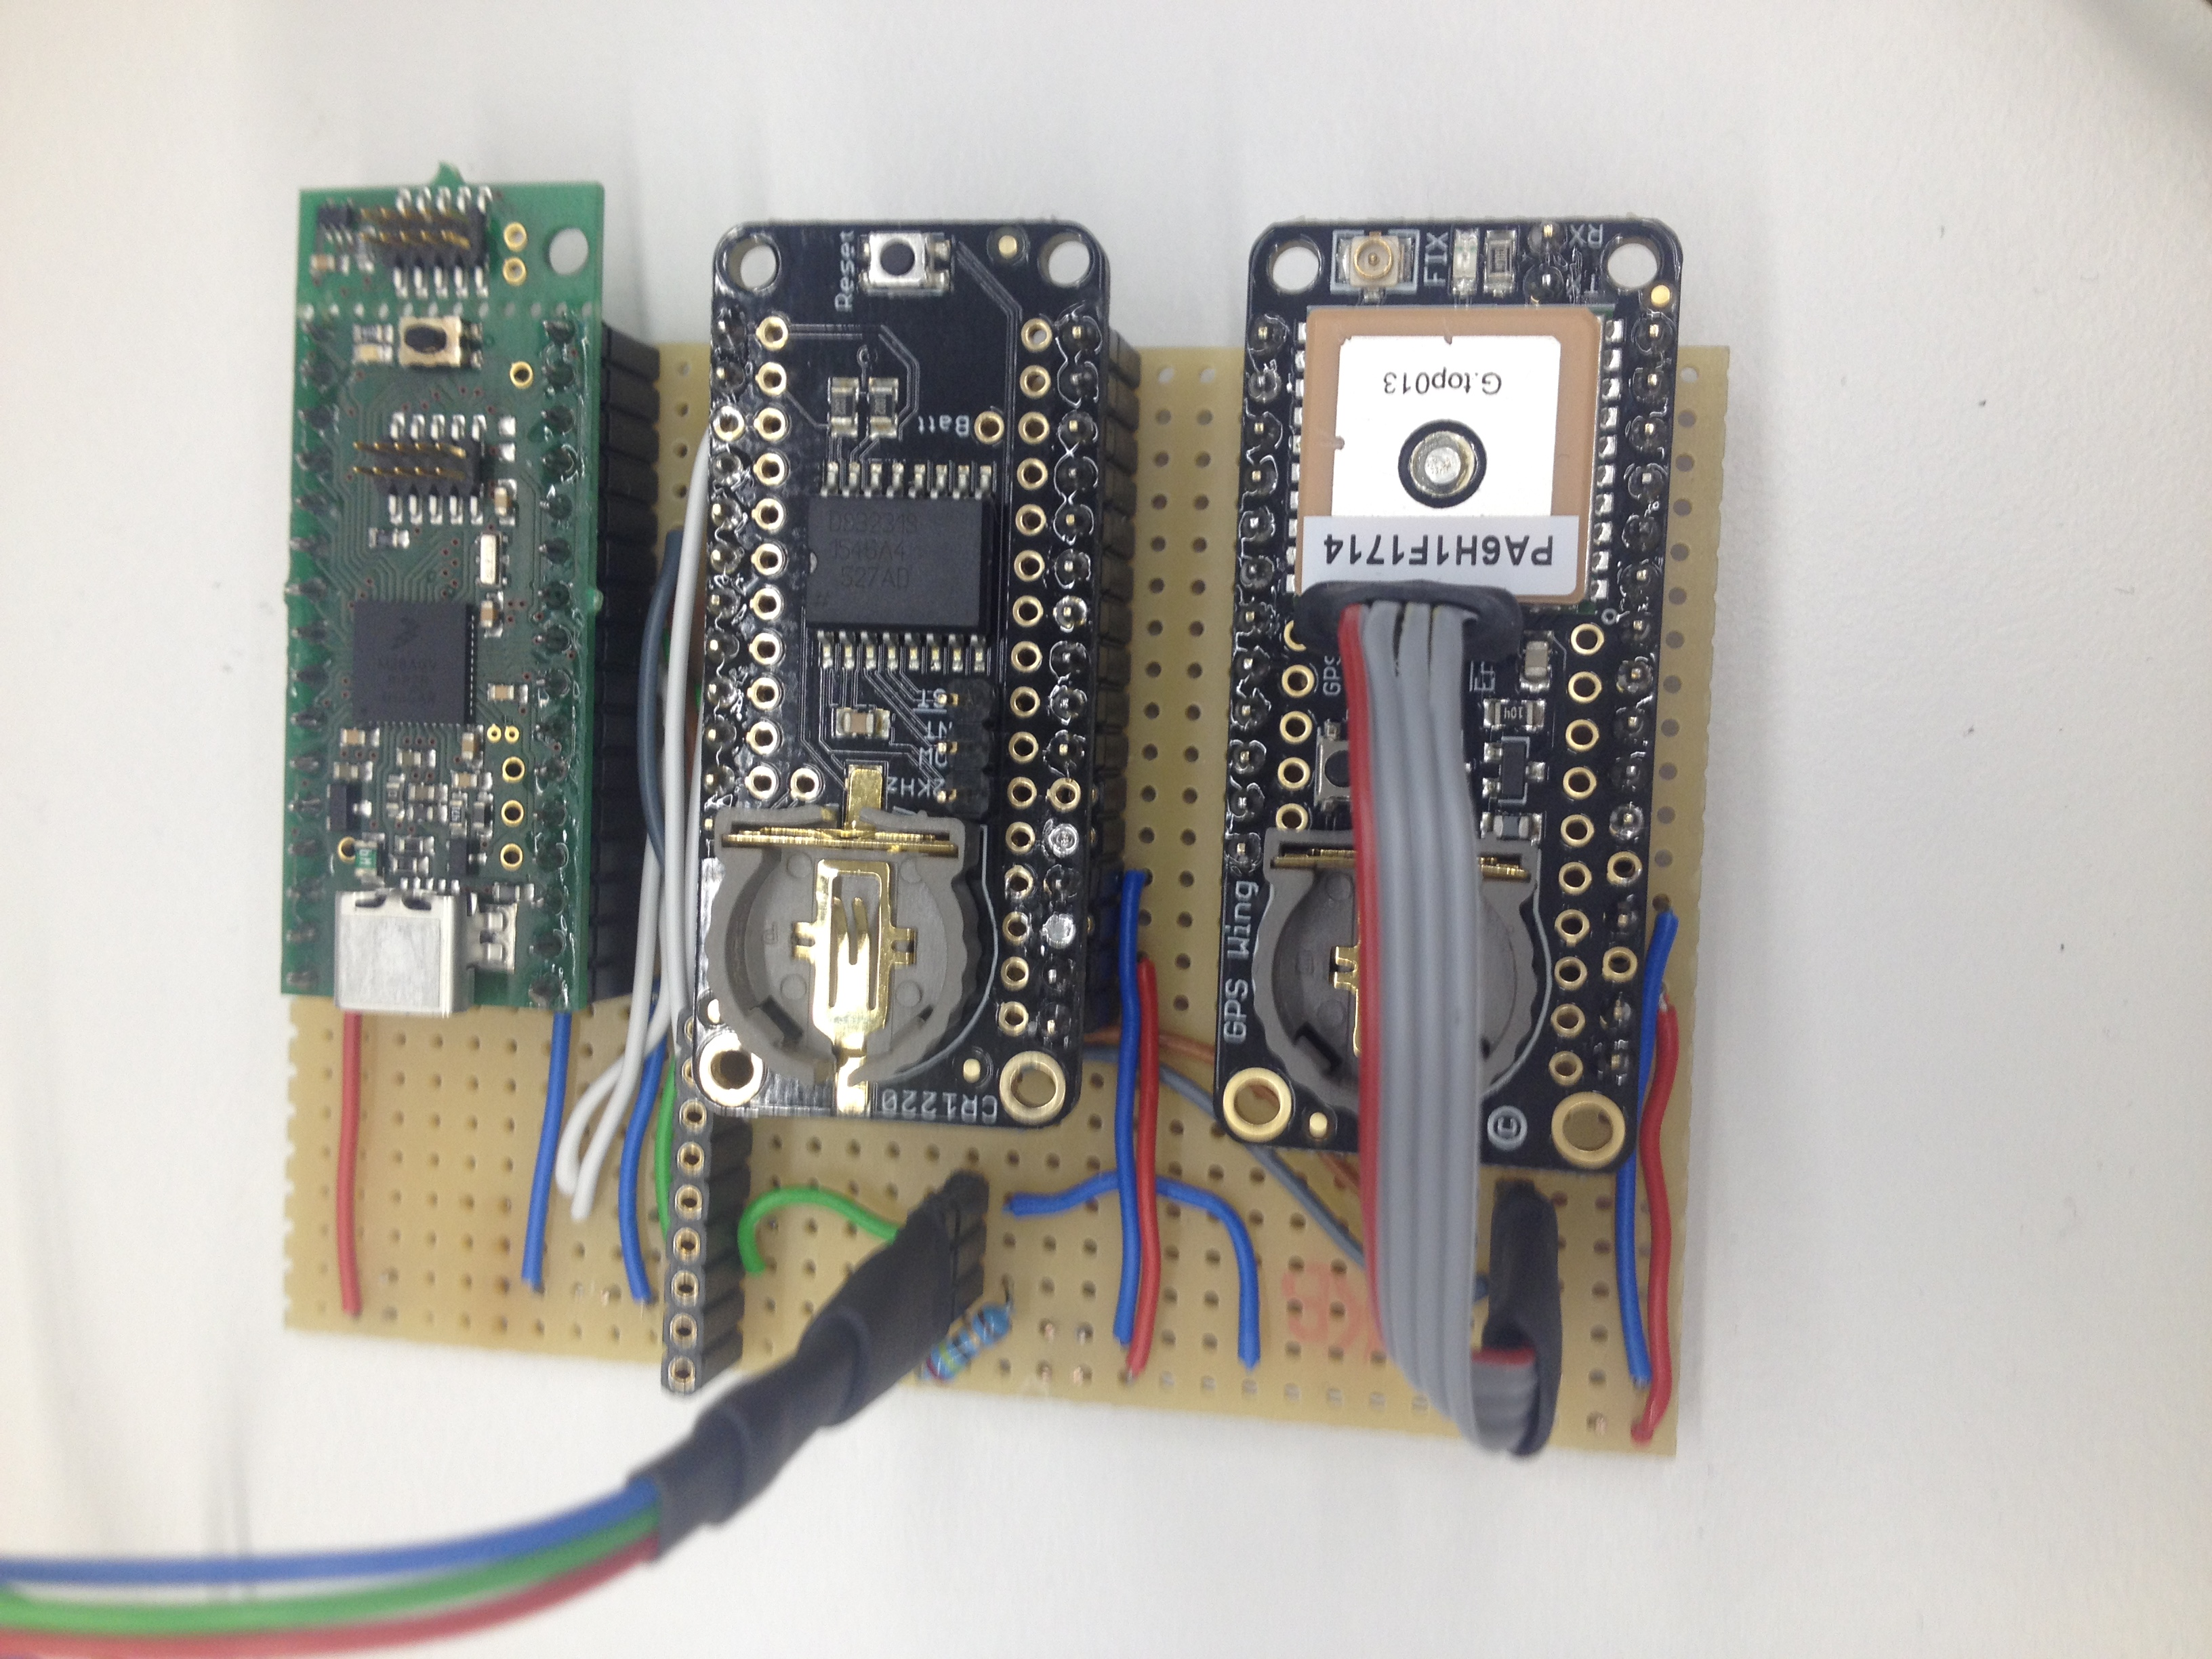
\includegraphics[width=.7\textwidth]{HW_Board_Complete}
		\caption{Gesamtanordnug der Hardware-Komponenten}
		\label{fig:hardware_board}
	\end{figure}
        \clearpage
        %!TEX root = SysSpec_ClockPendulumAnalyzer.tex
\subsection{Umsetzung der Datenpersistenz}
    Hier stehen Details zur Umsetzung der Datenspeicherung auf dem Raspberry Pi.
    \subsubsection{Datenspeicher}
    Da das Operationssystem des Raspberry Pi auf einer SD Karte gespeichert ist, empfiehlt es sich eine Alternative zu finden. SD Karten sind nicht für häufige Schreibzyklen ausgelegt. Für den Clock Pendulum Analyzer wird deshalb ein USB Speicher verwendet. Auf diesem wird die ganze Datenbank abgelegt.\\
    Der Datenspeicher wird beim Autostart über die \textit{/etc/fstab} Datei automatisch eingebunden.
    
    \subsubsection{SQLite als Datenbank}
    C++ bietet eine grosszügige Schnittstelle für SQLite Datenbanken. Durch SQLite braucht die Applikation auch keine umständliche Datenbankinstallation wie es bei MySQL der Fall wäre, da SQLite nur normale Dateien zum Aufbau verwendet.
    
    \subsubsection{Architektur und Beispielverwendung}
    Die Software speichert die folgenden Daten in einer einzelnen Tabelle ab.
    \paragraph{clock:}
    Der Wert in \textit{clock} hält den Namen fest der Uhr, von der die weiteren Daten stammen. Dieser wird beim Programmstart mitgeteilt.\\
    Das Feld ist vom Typ TEXT und besteht aus alphanumerischen Zeichen die der Regular Expression $$[a-zA-Z0-9]\{1,\}$$
    \paragraph{date:}\label{sec:db_date}%TODO datumsformat anpassen +zeit
    In diesem Feld steht der Zeitpunkt zu welchem der Datenwert entnommen wurde. Dazu wird die Systemzeit des RPi3 gespeichert und anschliessend so konvertiert, dass der Zeitstempel im Format \textbf{yyyyMMdd} gespeichert werden kann\\
    Das Feld ist vom Typ INTEGER und entspricht der Regular Expression
    $$[0-9]\{8\}$$
    \paragraph{absolutetime:}
    Hier steht der aktuell gemessene Zeitwert in absoluter Zeit. Der Wert bezieht sich auf die aktuell vergangenen Nanosekunden in einem Tag. Er startet bei 0:00 und läuft einen Tag.\\
    Das Feld ist vom Typ INTEGER und entspricht der Regular Expression
    $$[0-9]\{1,15\}$$
    \paragraph{heat:}
    Das Feld heat wird für den optionalen Teil Temperatureinfluss benötigt. Zum jetzigen Zeitpunkt ist dieses Feld mit 0 initialisiert.
    Das Feld ist vom Typ INTEGER und entspricht der Regular Expression
    $$[0-9]\{1,2\}$$
    \paragraph{humidity:}
    Das Feld humidity wird für den optionalen Teil Feuchtigkeitseinfluss benötigt. Zum jetzigen Zeitpunkt ist dieses Feld mit 0 initialisiert.
    Das Feld ist vom Typ INTEGER und entspricht der Regular Expression
    $$[0-9]\{1,2\}$$
    %TODO beispielverwendung einfügen
        \clearpage
        \subsection{Umsetzung des UI} %TODO UI Implementierung update nach Entwicklung
Die grafische Darstellung der ermittelten Messdaten wird in den folgenden Kapitel beschrieben.

\subsubsection{Webbrowser Client} 
Nach Aufgabenstellung wird ein web basierender Zugriff auf die ermittelten Messdaten gefordert. Dieser ist im Kontextdiagramm (Bild \ref{fig:kontext}) innerhalb der Systemgrenze als Web Client definiert.\\
Unter einem Web Client ist eine, auf dem Browser laufende Applikation zu verstehen.\\
\\
Der Zugriff auf die Messdaten läuft über die wohl definierte REST Schnittstelle, welche im Kapitel \ref{sec:rest} genauer erklärt ist. Dieser gekapselte Zugriff ermöglicht es eine unabhängige Darstellung zu implementieren.\\
Weiter gibt es die Möglichkeit andere grafische Benutzeroberflächen zu entwickeln, welche die gleichen Datengrundlagen haben.\\
\\
Der Aufbau des Clients erfolgt mittels eines Bootstrap Templates\footnote{Bootstrap Template von \cite{bootstrap}}. Im oberen Bereich wird die Temperatur, Feuchtigkeit, aktuelle Abweichung und Abweichung seit Beginn dargestellt. Darunter folgt ein Liniendiagramm, das den Ablauf der Abweichung pro Tag darstellt.Daneben ist eine Tagestabelle, die die Messergebnisse eines Tages anzeigt.\\
Das Liniendiagramm sowie die Tagestabelle können nach Datum gefiltert werden.

\begin{figure}[H]
    \centering
    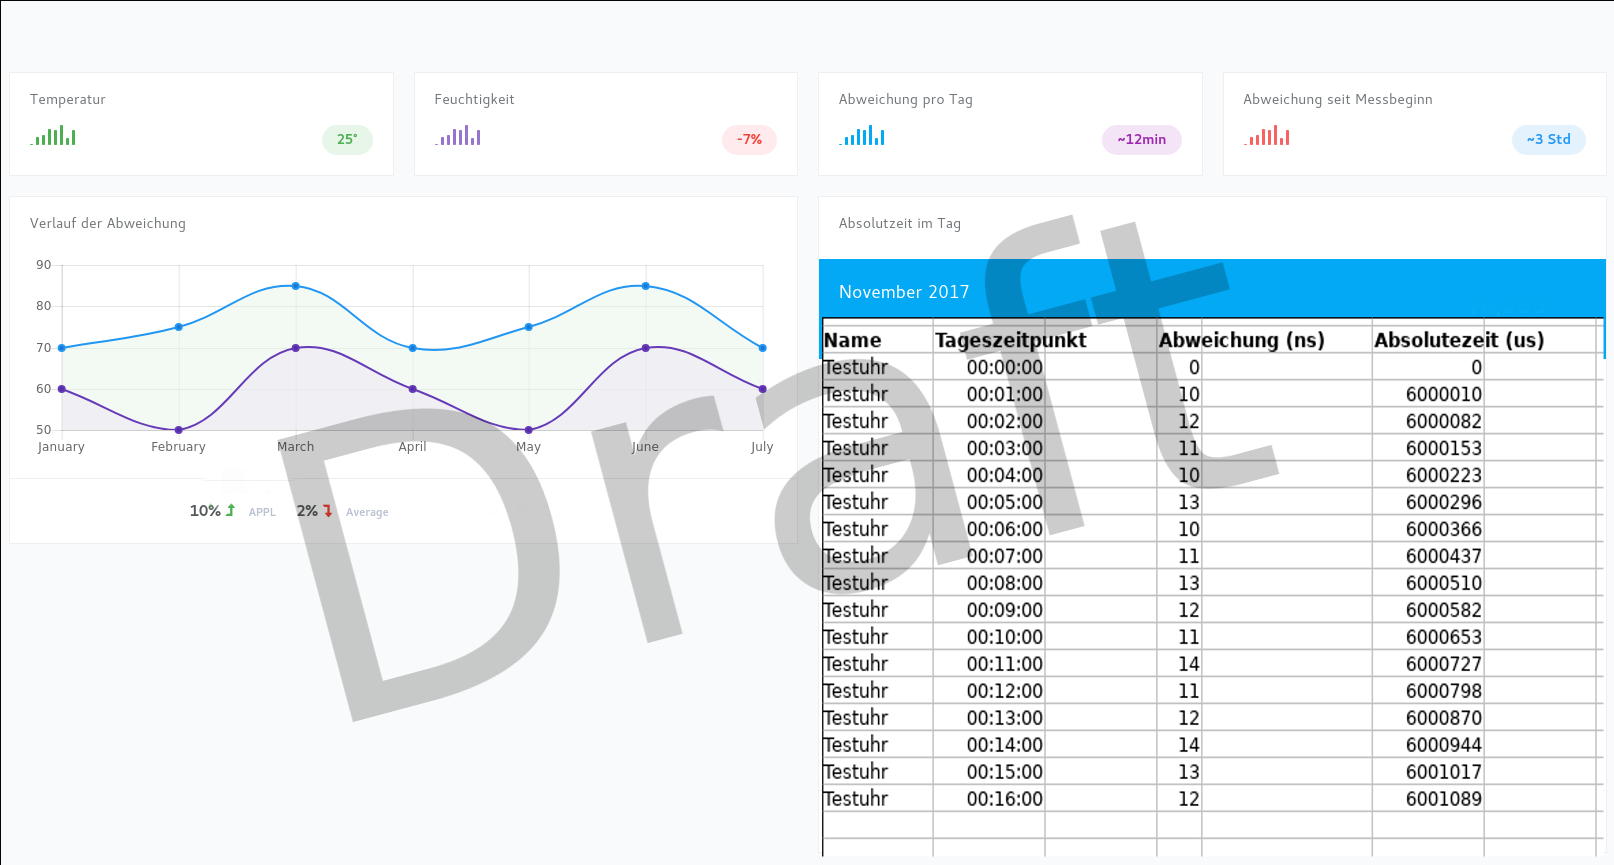
\includegraphics[width=\textwidth]{webclient_draft}
\end{figure}
        \clearpage
        %!TEX root = SysSpec_ClockPendulumAnalyzer.tex
\subsection{Sequenzdiagramm}
In diesem Kapitel werden einzelne Arbeitsabläufe anhand eines Sequenzdiagrammes dargestellt.
	\subsubsection{Start und Speichern einer Datenmessung}
    Dieses Sequenzdiagramm (Abbildung \ref{fig:sequence_save}) zeigt den Ablauf der Hauptfunktionalität.
    Zuerst werden alle zusätzlich benötigten Teilnehmer gestartet.
    Danach beginnt der Speichervorgang einzelner Datenmessungen.
    Dabei ruft das Programm die FIFO\footnote{First In, First Out}-Liste ab, welche durch die UART Kommunikation mit Messwerten befüllt wird.
    Sind 5 Datentupel aus der FIFO Liste gelesen, werden diese in der Datenbank gespeichert.
    \begin{figure}[H]
        \centering
        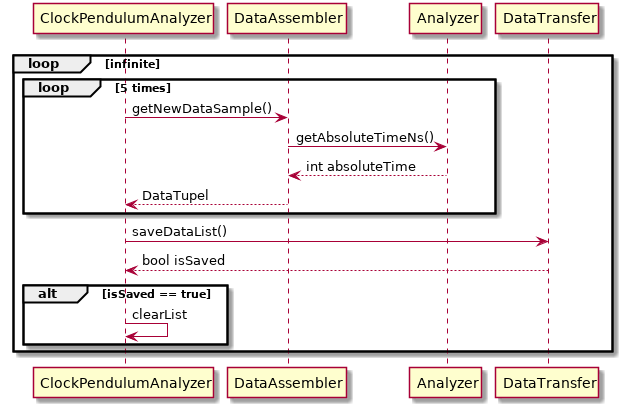
\includegraphics[width=\textwidth]{sequence_data_save.png}
        \caption{Sequenzdiagramm zum Speichern der Daten}
        \label{fig:sequence_save}
    \end{figure}

    \clearpage
    \subsubsection{Abrufen einer Datenmessung}
    Ein Webclient ruft Daten über eine HTTP Request auf die angebotene REST Schnittstelle.
    Als Antwort erhält er eine JSON Struktur der Messdaten.
    Das ganze wird im Sequenzdiagramm (Abbildiung \ref{fig:sequence_get}) unten abgebildet (mit dem Uhrennamen-Parameter als Beispiel).
    \begin{figure}[H]
        \centering
        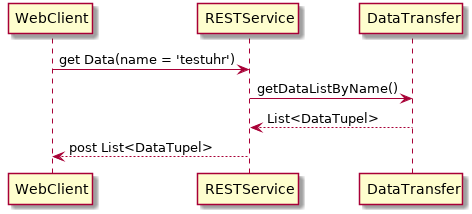
\includegraphics[width=.7\textwidth]{sequence_data_access.png}
        \caption{Sequenzdiagramm zum Aufrufen der Daten}
        \label{fig:sequence_get}
    \end{figure}
    %
	\subsubsection{Zählersystem}
	Die Software auf dem \hwb ist in C geschrieben und somit nicht objektorientiert. Dementsprechend sind die einzelnen Lebenslinien keine Objekte sondern eigene C-Dateien, deren Methoden entsprechend dem Diagramm aufgerufen werden. Die Akteure stellen dabei die Interrupt-Eingänge dar.
	\begin{figure}[H]
   		\centering
        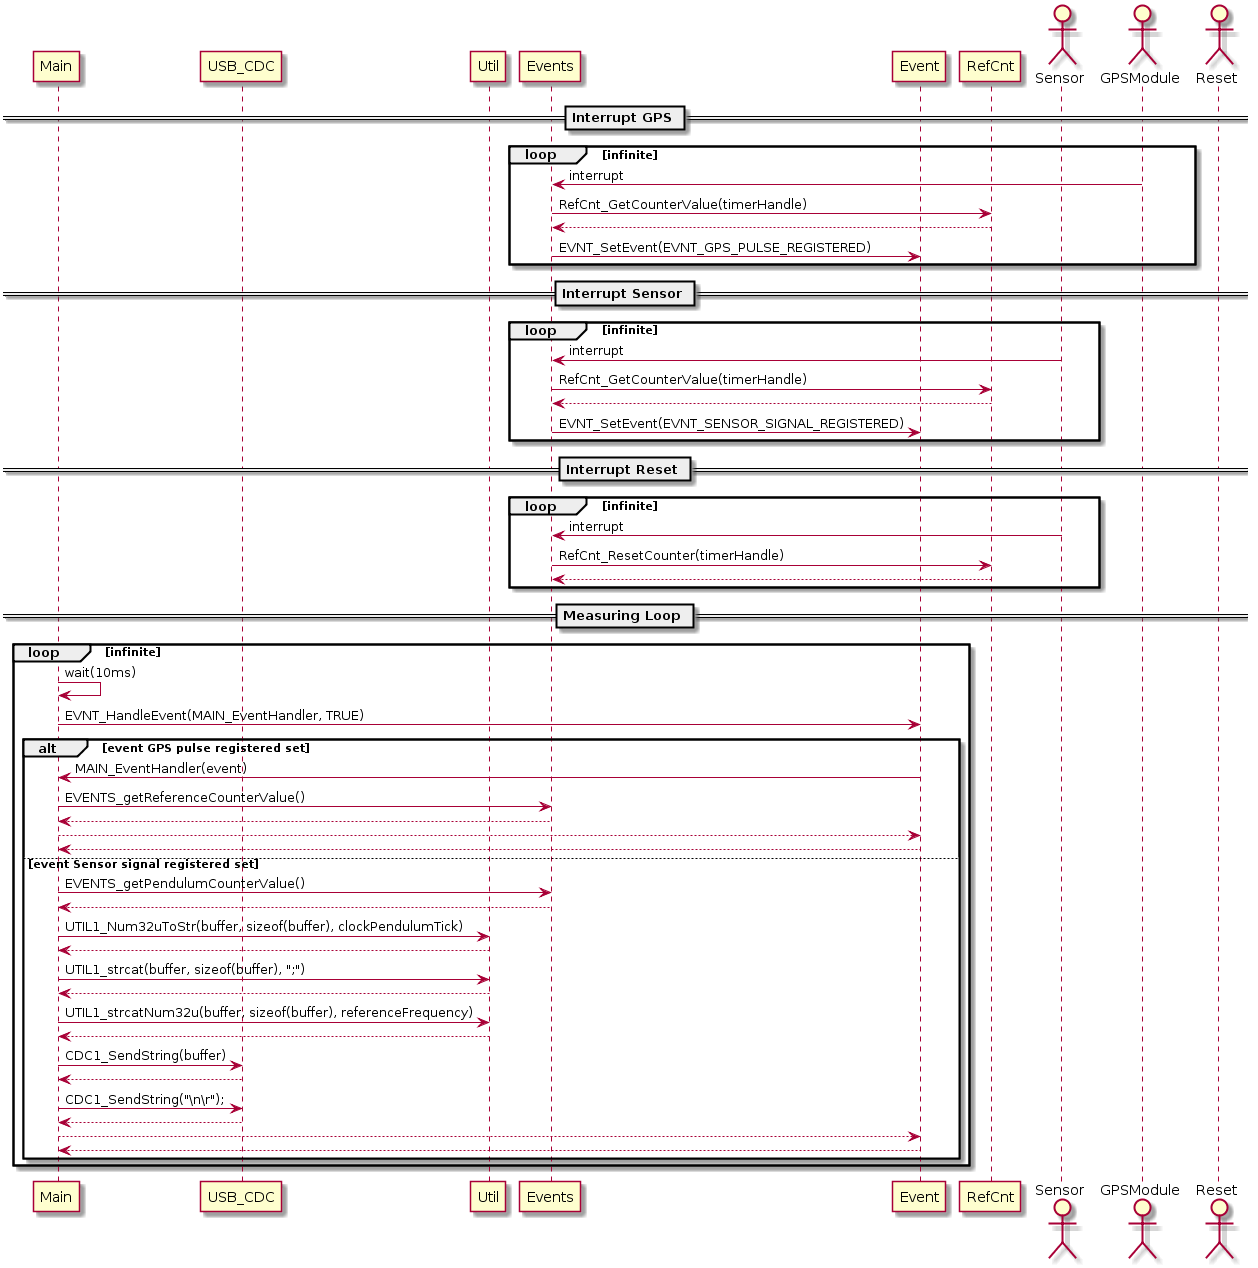
\includegraphics[width=.7\textwidth]{sequence_hwb.png}
        \caption{Sequenzdiagramm Zählersystem zur Pendelerfassung}
        \label{fig:sequence_hwb}
    \end{figure}
	\noindent Der Main-Loop, das eigentliche C-Programm, prüft alle 10 Millisekunden, ob ein Event gesetzt ist, oder ob noch Daten im USB-Kanal zum Senden vorhanden sind. Dementsprechend ist dieser Teil des Programmes nicht besonders zeitkritisch und kann problemlos zwischen den Interrupts durch das GPS-Modul und den Sensor verarbeitet werden.\\
	Die Interrupts des GPS-Moduls sind zeitkritisch und wie im Abschnitt \ref{cap:counter_realisation} beschrieben, von der höchsten Priorität. Da werden auch die aktuellen Zählerwerte umgehend gespeichert und anschliessend der entsprechende Event gesetzt, welcher dann beim nächsten Durchgang des Main-Loops verarbeitet wird. Der gesamte Ablauf ist im Sequenzdiagramm in Abbildung \ref{fig:sequence_hwb} dargestellt.

   	
        \clearpage
		%!TEX root = SysSpec_ClockPendulumAnalyzer.tex
\subsection{Klassendiagramm}
Die Klassen der Software arbeiten nach dem folgenden Klassendiagramm. Es umfasst eine Implementierung der REST Definition und Klassen für die Datenbankanbindung an SQLite.
\begin{figure}[H]
    \centering
    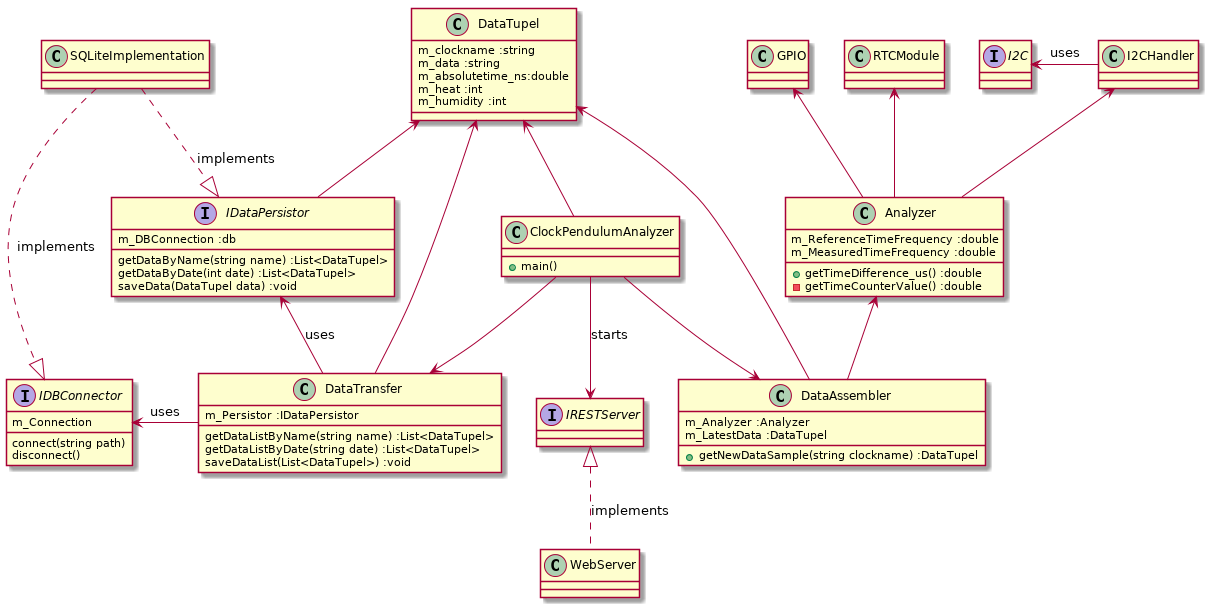
\includegraphics[width=\textwidth]{classdiagramm.png}
    \caption{Klassendiagramm der C++ Software auf dem Raspberry Pi}
\end{figure}
\subsubsection{Klassdetails}
    %TODO subject to change
	\begin{description}
        \item[ClockPendulumAnalyzer] Dies ist die Main Klasse. Sie startet alle Aufgaben.
        \item[I2CHandler] Diese Klasse öffnet und schliesst den $I^2C$-Bus und liest Daten von daran angeschlossenen Geräten.
        \item[GPIO] Eine Klasse die für das Arbeiten mit GPIO Pins auf dem Raspberry Pi zuständig ist.
        \item[Analyzer] Die Klasse ist für die Berechnung der Zeitdifferenz in Nanosekunden zuständig. Es kann auch die Differenz in Mikro- und Millisekunden ausgegeben werden.
        \item[DataAssembler] Die Klasse ist für das Zusammenfügen von Name (aus der Main Klasse) und den einzelnen Dateninputs aus dem Analyzer zuständig. Im Sequenzdiagramm ist dieser Ablauf dargestellt. 
        \item[DataTransfer] Diese Klasse ist für den Transport der DataTupel zwischen Webserver, Mainklasse und Datenbank zuständig.
        \item[DataTupel] Ein Daten Transfer Objekt (DTO) als Abstraktion der gemessenen Daten zu einem gegebenen Zeitpunkt. Beinhaltet Datum+Zeit, Name, Differenz und Werte für Feuchtigkeit und Wärme.
        \item[SQLiteImplementation] Die Implementierung der Schnittstelle \textit{IDataPersistor} und der \textit{IDBConnector} auf eine SQLite Umgebung.
    \end{description}
